\documentclass[12pt, a4paper]{article}
\usepackage[english, russian]{babel}
\usepackage[T2A]{fontenc}
\usepackage[utf8]{inputenc}
\usepackage[left=3cm,right=1.5cm,top=2cm,bottom=2cm,bindingoffset=0mm]{geometry}
\usepackage{titlesec}
\usepackage{amsmath}
\usepackage{setspace}
\usepackage[pdftex]{graphicx}
\usepackage{dsfont}
\usepackage{comment}
\usepackage[unicode, pdftex]{hyperref}
\usepackage{fancyhdr}
\usepackage{colortbl}
\usepackage{indentfirst}

\graphicspath{{C:/Users/9/Desktop/market_mod}}
\setlength{\parindent}{1.25cm}
\linespread{1.5}


\begin{document}

\pagestyle{fancy}
\fancyhf{}
\renewcommand{\headrulewidth}{0pt}

\begin{center}
САНКТ-ПЕТЕРБУРГСКИЙ ГОСУДАРСТВЕННЫЙ УНИВЕРСИТЕТ\\
Направление: 01.03.02 Прикладная математика и информатика \\
ООП: Прикладная математика, фундаментальная информатика и программирование \\
Кафедра технологии программирования \\

\vspace*{2cm}
\large \textbf{ОТЧЕТ О НАУЧНО-ИССЛЕДОВАТЕЛЬСКОЙ РАБОТЕ}
\end{center}
\vspace*{1.5cm}

\begin{flushleft}
\textbf{Тема задания:}
\end{flushleft}
\hspace{1cm} Исследование вероятностной модели предсказания лучшей цены в биржевом \\ стакане по трейдовым данным
\vspace*{0.5cm}

\begin{flushleft}
\textbf{Выполнил:}
\end{flushleft}
\hspace{1cm} Смирнов Алексей Артёмович, группа 21.Б02-пу 
\vspace*{0.5cm}

\begin{flushleft}
\textbf{Руководитель научно--исследовательской работы:}
\end{flushleft}
\hspace{1cm} Блеканов Иван Станиславович, кандидат технических наук, доцент, \\ заведующий кафедрой технологии программирования
 
 
\vspace*{7cm}
\begin{center}
САНКТ-ПЕТЕРБУРГ \\
2024
\end{center}

\newpage

\renewcommand{\contentsname}{\begin{center}Содержание\end{center}}
\tableofcontents

\newpage

\fancyfoot[C]{\thepage}

\section{Введение}

Одна из основных проблем любого участника рынка --- неполная информация о состоянии самого рынка. Соответственно, любой участник рынка желает получить как можно больше информации, на основе которой и будет принимать дальнейшие действия, так как чем большим объемом информации он владеет, тем более правильным будет само действие с точки зрения желаемых результатов. Для увеличения количества информации о рынке используют модели, которые основаны на том, что рынок есть сильно взаимосвязная система, поэтому, имея некоторую часть информации о состоянии системы, можно делать предположения о состоянии неизвестных частей системы по определенным законам, которые могут быть как строго математическими, так и эмпирическими.

Данная работа посвящена изучению одной вероятностной модели о биржевом стакане (Orderbook), где под термином биржевого стакана подразумевается некоторая рыночная структура, на которой взаимодействуют через посредника в виде биржи две стороны --- покупатели и продавцы. Более подробное описание биржевого стакана будет дано в разделе [000].

\subsection{Актуальность работы}
Изучаемая модель направлена на оценивание неизвестных, в определенный момент времени, параметров рынка, которые могут быть использованы для решения известной задачи Execution, которая является частью отрасли Financial Technologies, связанной с улучшением и оптимизацией финансовых услуг. Более формальное описание и обсуждение задачи Execution будет дано в разделе [000].

\subsection{Цели и задачи работы}
Основная цель работы --- оценить применимость предложенной модели, описать ситуации, при которых модель себя показывает лучше или хуже предполагаемого и, соответственно, определить практическую ценность данного статистического подхода.

\newpage

\section{Микроструктура биржевого стакана}

Биржа или биржевой стакан представляет собой две стороны рынка --- продавцов (ask сторона) и покупателей (bid сторона). Каждая сторона состоит из множества ценовых уровней (price levels), где каждый ценовой уровень является очередью заявок (orders) с фиксированными объемами (на ask стороне объем на продажу, на bid стороне объем покупки), порядок очереди определяется порядком появления заявок на бирже. Соответственно, лучшая цена на ask стороне называется лучшей ценой продажи, а лучшая цена на bid стороне, аналогично, называется лучшей ценой покупки.

\hypertarget{Orderbook}{
\begin{figure}[htbp]
\center{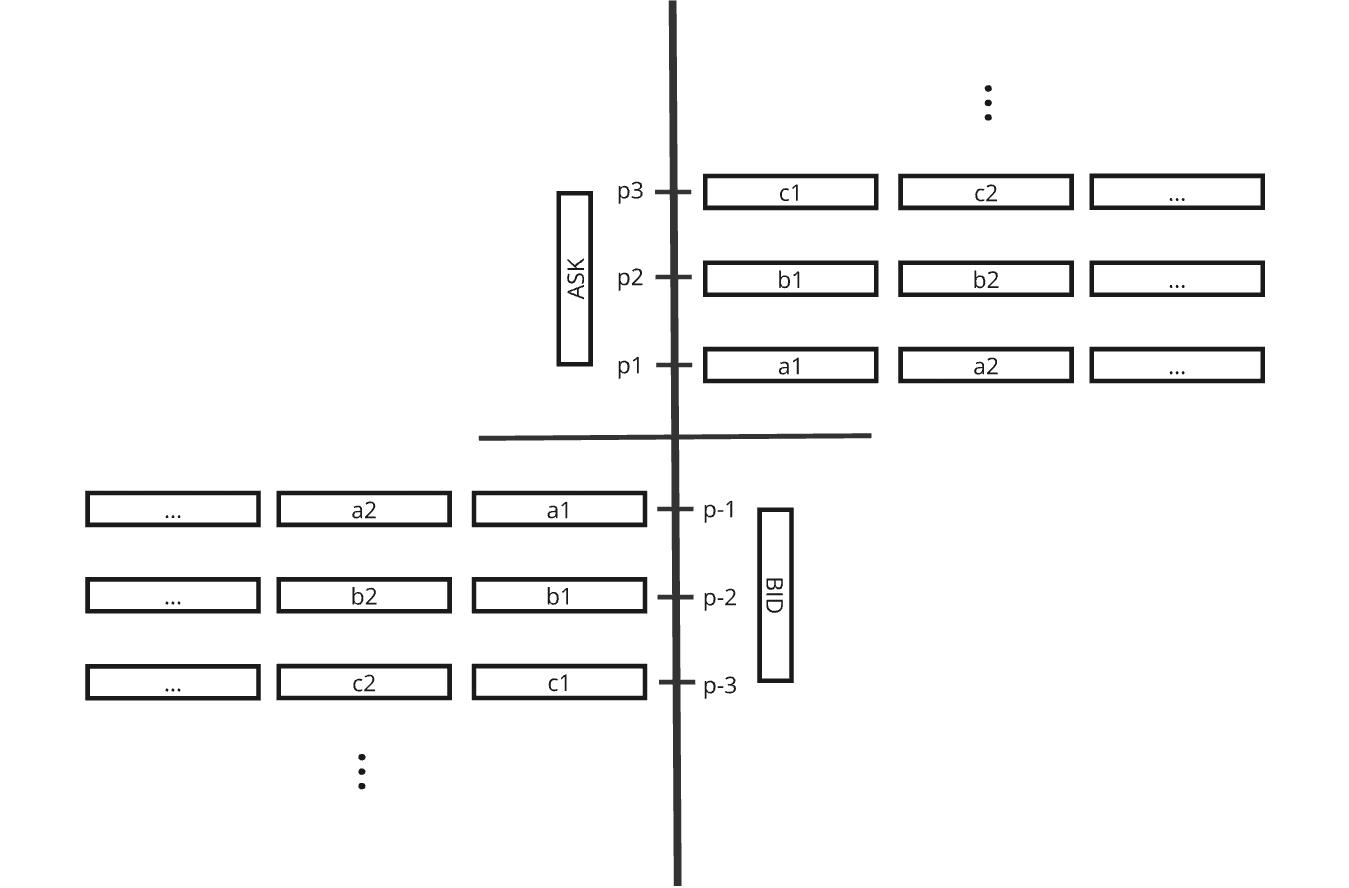
\includegraphics[width=1\textwidth]{Orderbook.png} Рисунок 1 --- Микроструктура биржевого стакана}
\end{figure}}

Как показано на $\hyperlink{Orderbook}{\text{Рисунке 1}}$, значения $p_i$ --- ценовые уровни, которые разбиты 
по объемам отдельных участников рынка, соответственно, общий объем, продающийся на конкретном уровне, есть сумма всех объемов в очереди.

\subsection{Основные характеристики биржевого стакана}

Величина $p_1 - p_{-1}$ есть величина спреда (spread), численно равный разности лучшей цены ask стороны и лучшей цены bid стороны, но имеющий прямое отношение к волатильности продукта, а именно, чем он больше, тем менее волатилен продукт. Это объясняется тем, что современная рыночная теория предполагает, что в каждый конкретный момент продукт имеет эталонную цену $(p_{ref})$, то есть истинную цену продукта в данный момент времени, купив или продав продукт по этой цене участник рынка считает, что он ничего не потерял и ничего не приобрел, следовательно желание продавцов --- продать продукт по большей цене, чем та, которую они считают для себя $p_{ref}$, а желание покупателей --- купить продукт дешевле, чем их субъективное представление о значении $p_{ref}$. Получаем, что значение $p_{ref}$ должно лежать в промежутке между лучшими ценами в стабильном состоянии биржевого стакана, так как иначе будет существовать такой ценовой уровень, по которому участники рынка будут считать выгодным для себя заключить сделку и, следовательно, этот ценовой уровень исчезнет. Очевидно, что ни один участник рынка точно не может знать значение $p_{ref}$, но каждый знает, что это значение находится внутри спреда и каждый участник рынка имеет ожидания по его движению в сторону увеличения или уменьшения, поэтому, если продукт является высоковолатильным, то частота сделок позволяет всем участникам рынка уточнить значение $p_{ref}$ и иметь более точные представления о его движении на коротких промежутках времени. Это означает, что интервал возможных значений $p_{ref}$ уменьшается для всех участников рынка, из-за чего ценовые уровни могут существовать довольно близко к истинному значению $p_{ref}$, так как не находится достаточное количество участников рынка, для которых данный уровень принадлежит их ожидаемому интервалу возможных значений $p_{ref}$. Иными словами, спред есть ожидаемый интервал возможных значений $p_{ref}$, согласованный всеми участниками рынка и ,как было показано выше, для высоковолатильных продуктов характерно иметь меньшую величину спреда, чем для низковолатильных, у которых участники рынка имеют меньше информации о значении $p_{ref}$ и, соответственно, ожидаемый интервал возможных значений $p_{ref}$ больше, то есть величина спреда больше.

Также стоит упомянуть, что на практике все численные значения на бирже принимают дискретные значения и величина между соседними значениями есть тик (tick). Например, для вычисления среднего значения цены продукта $(p_{mid})$, которую часто использую для оценки $p_{ref}$, применяют следующую формулу $\hyperlink{qrm}{[1]}$:

\[
\left\{
\begin{array}{cc}
\displaystyle \frac{p_1 + p_{-1}}{2} \quad \quad & if \quad \displaystyle\frac{p_1 + p_{-1}}{2} \notin \mathds{Z} \cdot t, \\
\displaystyle \frac{p_1 + p_{-1}}{2} \pm \frac{t}{2} \quad \quad & if \quad\displaystyle \frac{p_1 + p_{-1}}{2} \in \mathds{Z} \cdot t
\end{array}\right.,
\eqno(1)
\hypertarget{1}
\]
где $t$ - величина тика ценовых уровней. Суть формулы $\hyperlink{1}{(1)}$ в том, что значение $p_{ref}$ должно быть недостижимым значением ценового уровня для участников рынка, так как в противном случае все сделки происходили бы на этом уровне.

\subsection{Взаимодействие участников рынка на биржевом стакане}

Участники биржевого стакана имеют несколько инструментов взаимодействия между собой, а именно, любой участник может отправить три вида заявок на биржу: CancelOrder, LimitOrder, MarketOrder. 

CancelOrder или заявка на отмену --- может отправить участник, у которого есть незакрытые заявки в биржевом стакане. Участник рынка посылает бирже данную заявку, указывая ценовой уровень и объем, после чего биржа, подтверждая валидность операции, производит снятие заявки.

MarketOrder или заявка на продажу/покупку --- может отправить участник, который хочет в кратчайшие сроки продать/приобрести товара фиксированного объема. Биржа, при получении MarketOrder, пытается удовлетворить желание участника по минимально возможной цене, то есть производит продажу/покупку по лучшим ценам на стороне, в случае, если объем заявки превышает объем лучшего уровня, то производятся сделки на следующем ценовом уровне, который считается новым лучшим уровнем. При проведении сделок создается трейд (trade), в котором указан ценовой уровень, объем и стороны сделки, которыми являются составитель заявки и участники стакана, чьи заявки были полностью или частично выполнены. На одном ценовом уровне трейды создаются с участниками в порядке их очереди на биржевом стакане.

LimitOrder или ограниченная заявка --- может отправить участник, указав продажу/покупку, ценовой уровень, объем и тип заявки. Стандартными\footnote[1]{На практике биржа может использовать дополнительные типы заявок, но данные типы считаются самыми распространенными, которые будут учитываться в данной работе.} типами заявок считаются: fill--or--kill(FOK), immediate--or--cancel(IOC), good--till--cancel(GTC). 

Если LimitOrder имеет тип GTC, то биржа, получив данную заявку, попытается ее немедленно полностью или частично выполнить, то есть, если на данном ценовом уровне или ниже присутствуют заявки противоположной стороны суммарного объема не меньшего, чем указано в заявке, то заявка тут же исполняется, создаются трейды по алгоритму описанному выше, если же суммарного объема недостаточно, то заявка исполняется частично, на весь подходящий объем, при этом, биржа гарантирует, что цена всех сделок не выше, чем та, которую указал составитель в заявке, а оставшийся невыполненный объем заявки помещается в биржевой стакан на указанный ценовой уровень в конец очереди. Тип GTC выбирают те участники, которые не против того, что их заявка окажется в биржевом стакане, пока она не выполнится. 

Если LimitOrder имеет тип IOC, то происходят все вышеописанные действия для типа GTC, но, если возникает ситуация, когда заявка выполнилась на максимально возможный объем по цене, не превышающей указанную в заявке, то весь остальной объем возвращается участнику, не вставая в очередь и, соответственно, в биржевой стакан. Тип IOC выбирают те участники, которые согласны на частичное выполнение заявки в данный момент времени, но не хотят участвовать в биржевом стакане.

Если LimitOrder имеет тип FOK, то происходят все те же действия, но если возникает ситуация, что заявка не может быть исполнена в данный момент времени, то ее выполнение полностью отменяется. Тип FOK выбирают те участники, которых удовлетворяет только полное выполнение заявки в данный момент времени без участия в биржевом стакане.

Как видно, CancelOrder никогда не создают трейды, MarketOrder гарантированно создают трейды, а LimitOrder лишь в определенных ситуациях, что будет крайне важно для дальнейших исследований модели, а также то, что трейды всегда происходят по лучшим ценам.

\subsection{Практические особенности получения данных с бирж}

Как было сказано ранее, каждый участник рынка желает получить полную информацию о самом рынке, но данное желание не может быть реализовано даже технически, так как, когда на бирже произошло какое-то событие, которое она транслирует через известные участникам информационные каналы, из-за задержек каналов у участников нет никаких гарантий, что за время прохождения информации по каналу, внутри биржи не было обработано другое событие и их представление о состоянии рынка является актуальным. Одновременно с этим, задержка получения информации у разных участников отличается, из-за чего в определенные моменты нарушается симметрия информации участников рынка, что противоречит постулатам идеального рынка, на которых основан непрерывный аукцион двойной цены применяемый большинством бирж.

Для того, чтобы избежать малейших рассинхронизаций внутри биржи, все изменения состояния биржи происходят линейно, то есть однопоточно, по внутреннему времени этого потока и определяется точное время любых изменений.

Рассмотрим пример работы с биржей на примере криптовалютной биржи BINANCE, а именно через предоставляемый самой биржей BINANCE API $\hyperlink{binance_api}{[2]}$. 

BINANCE API имеет свой протокол REST API для получения различной информации, но в данной работе рассмотрим только Market Data endpoints, который возвращает снепшот (sneapshot), то есть полное состояния биржевого стакана конкретного продукта, но у него есть ряд ограничений, одно из которых --- частота отправки запроса, которая является хоть и динамической, то есть биржа ответом на запрос также возвращает временной промежуток, который требуется выждать, чтобы выслать следующий запрос, но в рамках частоты торгов на данной криптобирже является очень большим ограничением, так как среднее время между запросами составляет несколько минут, то есть только по данной информации невозможно следить за состоянием биржевого стакана в реальном времени и предпринимать какие-либо действия. Еще одним недостатком является отсутствие у снепшота времени отправки (vanue tamestamp), то есть по ответу биржи невозможно определить задержку канала связи, но у снепшота есть параметр --- конечный id события, которое было учтено в данном снепшоте, соответственно, если получать все события происходящие на бирже, то сравнивая их id и конечный id снепшота, то можно восстановить момент в который был отправлен снепшот, так как биржа гарантирует последовательное инкрементальное увеличение id всех событий происходящих на бирже в силу однопоточности ядра.

У BINANCE API есть соответствующие Web Socket Streams (WSS) различных типов по каждому продукту. В данной работе рассмотрим два типа: Trade Stream и Diff. Depth Stream. Когда на бирже происходит трейд, то информация сразу же транслируется по Trade Stream с соответствующей информацией о произошедшей сделке, в том числе время трейда, которое может не совпадать со временем обработки события, которое породило данный трейд, так как формирование трейдов происходит параллельно с формированием иной информации о произошедшем событии, следовательно, время трейда есть внутреннее время данного потока, которое может отличаться от времени любого другого потока. Транслирование событий (Depth), в которых записаны все изменения биржевого стакана с момента последнего Depth, в Diff. Depth Stream происходит по времени, можно получать событие каждые 100 или 1000 миллисекунд, что также довольно медленно для высокочастотной торговли. Благодаря одному снепшоту из Market Data endpoints и постоянному получению Depth из Diff. Depth Stream и накладыванию этих изменений на локальный биржевой стакан, можно получать актуальное состояние биржевого стакана каждые 100 миллисекунд. 

Аналогично, можно накладывать на локальный биржевой стакан и все трейды из Trade Stream, хоть это не даст полного актуального состояния из-за того, что нетрейдовые события будут учтены только в Depth, но даст возможность поддерживать некоторую актуальность лучших цен, хотя не гарантированную. 

Стоит отметить, что в снепшотах, Depth и трейдах объемом обозначается общий объем ценового уровня, без разделения по участникам, то есть, даже если теоретически поддерживать актуальный биржевой стакан в любой момент времени по данным событиям, то у нас все равно не будет полного состояния биржевого стакана.

Теоретически может возникнуть проблема с синхронизацией событий с разных WSS, которые формируют разные потоки биржи, то есть возможна ситуация, когда события с разных потоков придут не в том порядке, в котором они были отправлены биржей, а время отправления данных событий не может быть сравнено в силу отсутствия гарантий синхронизаций времени потоков, на этот случай можно полагаться на id событий, например Depth хранит два значения id --- начальный и конечный id учтенных событий, по которым можно восстановить его относительное расположение относительно других событий имеющих id из других WSS, но у BINANCE API существуют WSS, которые невозможно синхронизировать с другими, например, Individual Symbol Book Ticker Streams, в котором отправляются события, хранящие лучшие цены каждой стороны, а также его относительное расположение относительно других событий с данного WSS, следовательно, у нас никакой информации для синхронизации событий с данного WSS и любого другого WSS.

\section{Модель}

\subsection{Задача Execution}

Известная задача Execution может формулироваться в нескольких вариациях, например, пусть в данный момент времени пришел сигнал, после которого нужно купить максимальное количество товара на фиксированное количество денег за фиксированное время, или, например, пусть в данный момент времени пришел сигнал, после которого нужно купить фиксированное количество товара за минимальное количество денег за фиксированное время. В данной работе под задачей Execution будет подразумеваться вторая формулировка задачи.

Как видно из формулировки, исполняющий заявку на Execution должен быть готов выполнить в любое время, когда пришел сигнал, то есть нужно иметь возможность выполнять данную заявку даже не имея полной информации о состоянии рынка, при этом время на исполнение заявки может быть недостаточно, чтобы дождаться ситуации, когда исполняющий сможет получить хоть какую-то дополнительную информацию о состоянии рынка, поэтому данная задача требует выполнить заявку с информацией в момент сигнала, а, так как сигнал может прийти в любой момент времени, то, следовательно, требуется знать необходимые параметры состояния рынка для принятия решений в любой момент времени, именно для предсказания одного из таких параметров и предлагается вероятностная модель, которая будет описана ниже.

\subsection{Построение модели}
 
Предлагаемая модель основывается на некоторых эмпирических вероятностных распределениях определенных параметров биржевого стакана, а именно:

\begin{enumerate}
\item Время между трейдами распределено по экспоненциальному закону распределения, то есть мы считаем, что участники рынка торгуют и не торгуют в одни и те же моменты времени, можно сказать, что происходят всплески активности трейдов, которые образуют некоторые группы, разделенные меньшей активностью ($\hyperlink{trade_exp}{\text{Рисунок 2}}$).

\item Абсолютное отклонение цены в биржевых событиях от лучшей цены на соответствующем уровне распределено по Пуассоновскому распределению, что естественно предложить, ведь все трейды происходят на лучших ценах, соответственно, абсолютное смещение лучшей цены распределено по Пуассоновскому распределению, которое является дискретным, что хорошо описывает практическую сторону реализации хранения чисел биржей, как было показано в конце параграфа 2.1.
\end{enumerate}

Модель будет предсказывать смещение лучшей цены одной стороны по данным полученным по трейдам, то есть по ряду лучших цен, ряду времени между трейдами и прошлой известной лучшей цене, то есть без учета объемов трейдов, путем построения доверительной области (в нашем случае двумерной) с учетом корреляции признаков, ведь как говорилось ранее --- биржевой стакан сильносвязная система, поэтому именно благодаря корреляции признаков модель будет учитывать время получения трейдов при определении доверительного интервала для смещения лучшей цены. 
\newpage
Для определения многомерной доверительной области среднего значения зависимых нормально распределенных случайных величин используют обобщенную статистику Стьюдента $t^2$ --- статистику Хотеллинга $T^2$ $\hyperlink{hotteling}{[3]}$ ($\hyperlink{inter}{\text{Рисунок 3}}$).
	
\begin{figure}[h]
\begin{minipage}[h]{0.5\linewidth}
\center{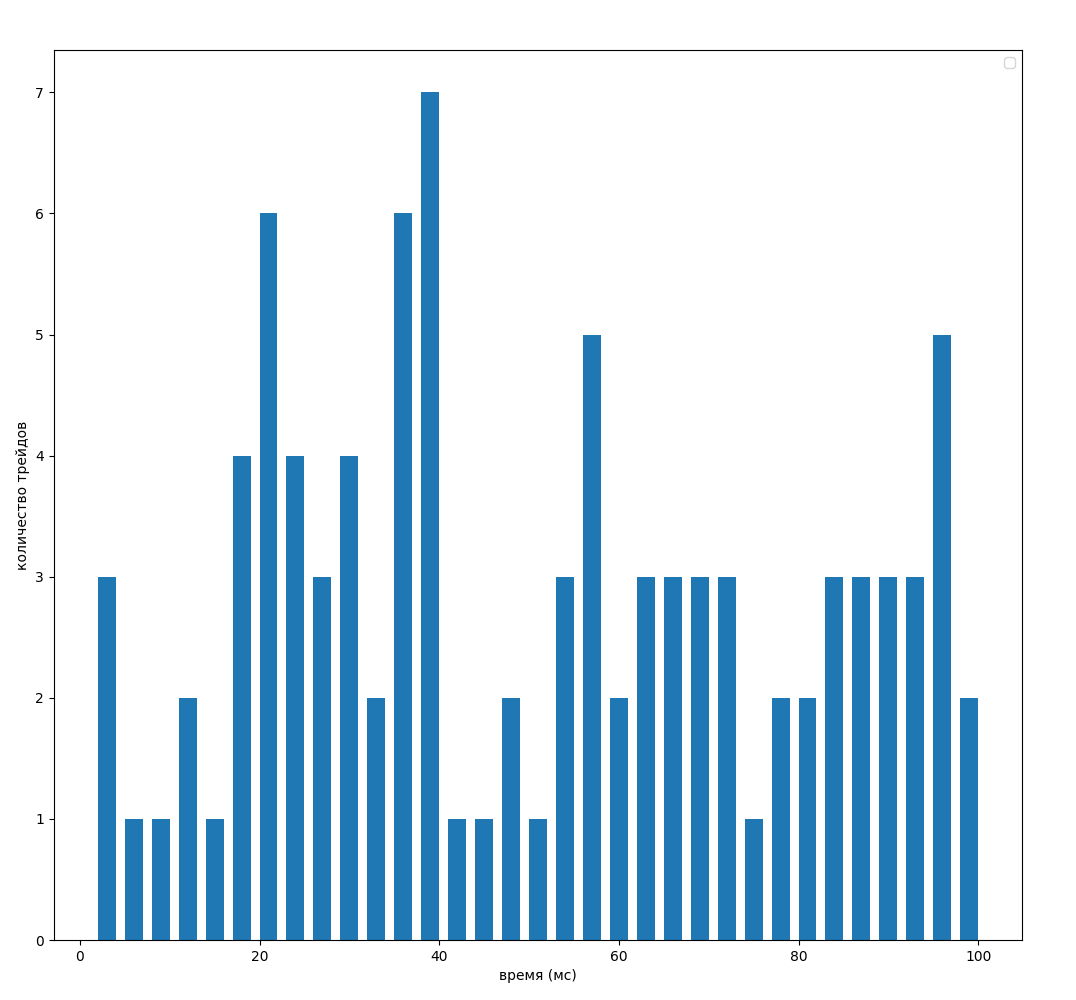
\includegraphics[width=1\linewidth]{trade_exp.png} \\ \hypertarget{trade_exp}{Рисунок 2 --- Симулированное распределение трейдов}}
\end{minipage}
\hfill
\begin{minipage}[h]{0.5\linewidth}
\center{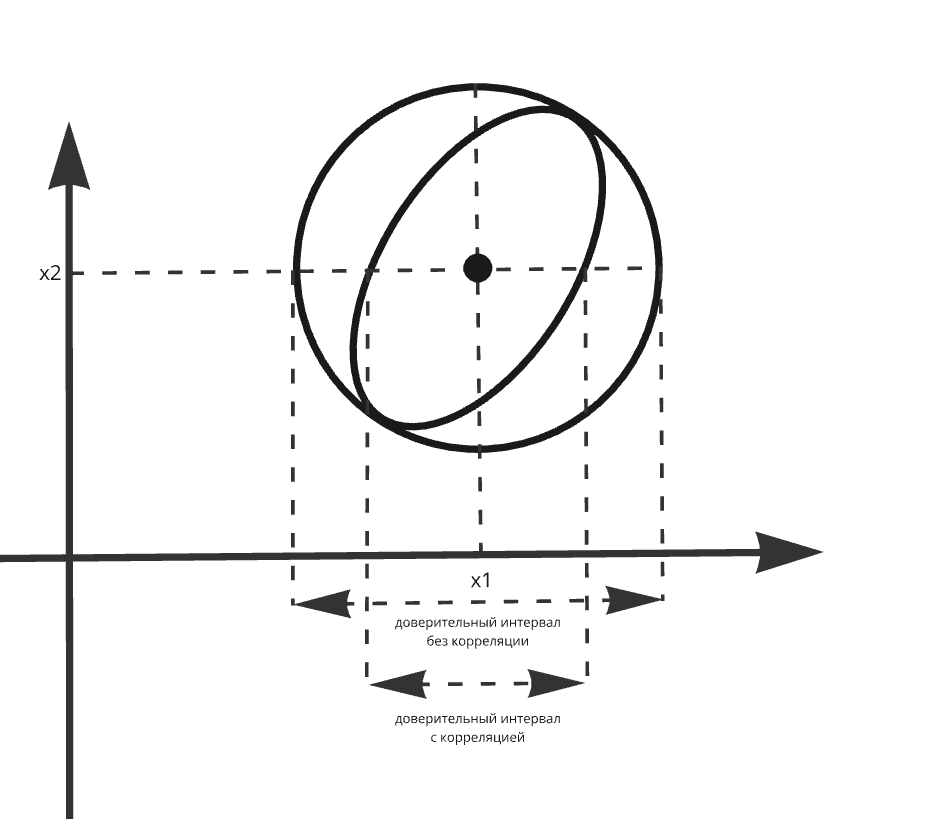
\includegraphics[width=1\linewidth]{inter.png} \\ \hypertarget{inter}{Рисунок 3 --- Уменьшение условного доверительного интервала при использовании учета корреляции признаков}}
\end{minipage}
\label{ris:image1}
\end{figure}

Пусть имеется $n$ измерений каждой из $k$ одномерной нормально распределенной случайной величины, которые могут быть зависимы между собой, тогда доверительная область с вероятностью $p$ для $k$-мерного вектора средних значений $\mu$ есть $k$-мерный эллипсоид, который задается следующим выражением:
\[
T^2 \geq n (\overline{X} - \mu)^TC^{-1}(\overline{X} - \mu),
\eqno(2)
\]
где $C$ --- матрица $k \times k$ выборочных оценок ковариаций, $\overline{X}$ --- выборочная оценка вектора средних значений, $T^2$ --- статистика Хотеллинга, равная $\displaystyle \frac{k(n-1)}{n-k}F^p_{v_1, v_2}$, где $F^p_{v_1, v_2}$ --- квантиль распределения Фишера с вероятностью $p$ и степенями свободы $v_1 = k, v_2 = n - k$. Так как нас интересуют только доверительный интервал для одной компоненты (Н.У.О для компоненты $\mu_k$) вектора средних значений, то мы полагаем все остальные компоненты равные выборочным оценкам $\mu_i = \overline{X}_i \;\forall i = \overline{1,k-1}$, то есть сечем $k$-мерный эллипсоид одномерной прямой, проходящей через его центр и параллельной оси $k$-той компоненты. 

\newpage
Соответственно получаем:

\[
\begin{array}{c}
\displaystyle \frac{k(n-1)}{n(n-k)}F^p_{k, n-k} \geq c_{kk}(\overline{X_k} - \mu_k)^2 \Rightarrow \\
\\
\Rightarrow \displaystyle \overline{X_k} - \sqrt{\frac{1}{c_{kk}}\frac{k(n-1)}{n(n-k)}F^p_{k, n-k}} \leq \mu_k \leq \overline{X_k} + \sqrt{\frac{1}{c_{kk}}\frac{k(n-1)}{n(n-k)}F^p_{k, n-k}} \:,
\end{array}
\hypertarget{3}
\eqno(3)
\]
где $c_{kk}$ --- элемент $k$-той строки и $k$-того столбца обратной матрицы выборочных оценок ковариации. Для случая $k=2$, который будет представлен в данной работе, значение $c_{22}$ определяется как: 
\[
\displaystyle c_{22} = \frac{cov(\xi_1, \xi_1)}{cov(\xi_1, \xi_1)cov(\xi_2, \xi_2) - cov(\xi_1, \xi_2)^2},
\eqno(4)
\] 
где $cov$ --- значение выборочной ковариации, $\xi_1$ --- генеральная совокупность для значений интервалов времени между трейдами, $\xi_2$ --- генеральная совокупность для значений смещения лучшей цены в трейдах.

По формуле $\hyperlink{3}{(3)}$ можно рассчитать доверительный интервал для среднего значения нормально распределенной величины, но в начале данного параграфа были выдвинуты предположения о распределении исследуемых величин, которые не являются нормальными, поэтому требуется провести нормализацию распределений, путем преобразования рассматриваемых значений.

Стандартным путем нормализации экспоненциально распределенной величины является ее логарифмирование, то есть вместо значений $\xi_1$ будут использоваться моделью значения $\ln(\xi_1)$, а для нормализации величины $\xi_2$, распределенной по Пуассоновскому распределению, часто берут ее корень, то есть $\sqrt{\xi_2}$, но, так как смещение лучшей цены может быть в обе стороны, то стоит учитывать знак значения. Соответственно, при получении трейда, который имеет ценовой уровень $p_t$ и интервал времени между ним и прошлым событием $t$, и известной информации о прошлой лучшей цене $p_{best}$ соответствующей стороны, будут формироваться значения $\ln(t), \text{sign}(p_t - p_{best})\sqrt{|p_t - p_{best}|}$, которые будем считать нормально распределенными зависимыми случайными значениями.

Из неравенства $\hyperlink{3}{(3)}$:
\[
\displaystyle \overline{X_2} - \sqrt{\frac{1}{c_{22}}\frac{k(n-1)}{n(n-2)}F^p_{k, n-2}} \leq \text{sign}(\eta_2 - p_{best})\sqrt{|\eta_2 - p_{best}|} \leq \overline{X_2} + \sqrt{\frac{1}{c_{22}}\frac{k(n-1)}{n(n-2)}F^p_{k, n-2}} \:,
\hypertarget{5}
\eqno(5)
\]
где $\eta_2$ --- среднее значение ценового уровня лучшей цены оцениваемой стороны.

Нетрудно показать, что:
\[
\displaystyle a \leq b \;\Leftrightarrow\; \text{sign}(a) \cdot a^2 \leq \text{sign}(b) \cdot b^2.
\hypertarget{6}
\eqno(6)
\]
Применяя дважды $\hyperlink{6}{(6)}$ к $\hyperlink{5}{(5)}$, получим:

\[
\begin{array}{c}
\displaystyle \text{sign}\left(\overline{X_2} - \sqrt{\frac{1}{c_{22}}\frac{k(n-1)}{n(n-2)}F^p_{k, n-2}}\right) \left(\overline{X_2} - \sqrt{\frac{1}{c_{22}}\frac{k(n-1)}{n(n-2)}F^p_{k, n-2}}\right)^2 \leq \\
\displaystyle \leq \text{sign}(\eta_2 - p_{best})|\eta_2 - p_{best}| \leq \\
\displaystyle \leq \text{sign}\left(\overline{X_2} + \sqrt{\frac{1}{c_{22}}\frac{k(n-1)}{n(n-2)}F^p_{k, n-2}}\right) \left(\overline{X_2} + \sqrt{\frac{1}{c_{22}}\frac{k(n-1)}{n(n-2)}F^p_{k, n-2}}\right)^2,
\end{array}
\eqno(7)
\]
и, заменяя $\text{sign}(\eta_2 - p_{best})|\eta_2 - p_{best}| = \eta_2 - p_{best}$, получаем окончательную оценку доверительного интервала для среднего значения лучшей цены $\eta_2$:

\[
\begin{array}{c}
\displaystyle p_{best} + \text{sign}\left(\overline{X_2} - \sqrt{\frac{1}{c_{22}}\frac{k(n-1)}{n(n-2)}F^p_{k, n-2}}\right) \left(\overline{X_2} - \sqrt{\frac{1}{c_{22}}\frac{k(n-1)}{n(n-2)}F^p_{k, n-2}}\right)^2 \leq \\
\displaystyle \leq \eta_2 \leq \\
\displaystyle \leq p_{best} + \text{sign}\left(\overline{X_2} + \sqrt{\frac{1}{c_{22}}\frac{k(n-1)}{n(n-2)}F^p_{k, n-2}}\right) \left(\overline{X_2} + \sqrt{\frac{1}{c_{22}}\frac{k(n-1)}{n(n-2)}F^p_{k, n-2}}\right)^2.
\end{array}
\hypertarget{8}
\eqno(8)
\]

Формулу $\hyperlink{8}{(8)}$ можно применять в любой момент времени, сохраняя информацию о происходящих ранее трейдах, то есть данная модель позволяет иметь интервальную оценку для лучшего ценового уровня в любой момент времени.

Конечно, данная оценка может быть посчитана только если произошли хотя бы три трейда на интересующей нас стороне, что делает ее применимой только для товаров имеющих уровень волатильности больше, чем некоторый минимально требуемый, но если, как в случае BINANCE, за 100 миллисекунд не произошло хотя бы три трейда, то можно считать, что лучшая цена товара не изменилась, хотя, конечно, возможно, что на рынке данного товара происходит огромное количество нетрейдовых событий, которые могли изменить лучшую цену на сколь угодно большое значение, но в данной работе считаем данный сценарий маловероятным, и в случае недостаточного количества трейдов будем считать, что модель предсказывает, что интервальная оценка вырождается в точечную, где среднее значение $\eta_2 = p_{best}$.

Из рассуждений выше об ограничениях применения модели сразу видны ее недостатки, а именно то, что учитываются только трейдовые события, а вклад нетрейдовых мы никак не можем даже оценить, но мы можем лишь надеяться на то, что при большом количестве нетрейдовых событий происходит и большое количество трейдовых, так как биржа сильносвязная система, благодаря которым мы может поддерживать актуальную оценку.

Насколько критичны недостатки модели и насколько адекватна реальности сама оценка лучше всего понять при  использовании данной модели на практике и сравнении истинного значения с предсказанными.

\section{Практические результаты}

В данной главе будет тестироваться модель предложенная выше путем сравнения полученного значения, истинного значения и эталонного значения, где эталонное значение --- значение, полученное без использования модели.

\subsection{Вероятностный симулятор взаимодействия участников \\ биржевого стакана}

Для проверки модели был построен симулятор биржевого стакана, где происходила полная искусственная вероятностная генерация всех взаимодействий участников биржи.


\begin{comment}
\section{Вероятностный симулятор взаимодействия \\ участников биржевого стакана}
\section{Практические результаты}

\hypertarget{qrm}
\hypertarget{binance_api}
\hypertarget{hotteling}
\end{comment}
\end{document}